\documentclass[10pt]{article}
\usepackage{amsmath, blindtext,hyperref}
\usepackage[utf8]{inputenx}
\usepackage[T1]{fontenc} 

\usepackage{graphicx, rotating} % Required for including images
\usepackage[font=small,labelfont=bf]{caption} % Required for specifying captions to tables and figures
\title{ INF368 Selected Topics in Machine Learning \\
		\huge Exercise 3: Siamese Networks and Zero Shot Learning}
\author{Håvard Vågstøl}
\makeatletter

\renewcommand\paragraph{%
    \@startsection{paragraph}{4}{0mm}%
       {-\baselineskip}%
       {.5\baselineskip}%
       {\normalfont\normalsize\bfseries}}

\renewcommand*\env@matrix[1][*\c@MaxMatrixCols c]{%
  \hskip -\arraycolsep
  \let\@ifnextchar\new@ifnextchar
  \array{#1}}
\makeatother
\begin{document}
\maketitle
\section{Abstract}
The exercise covers vector embedding of image data. Plankton images from the ZooScanNet data set are embedded to a 64 dimensional space using the provided neural network implementation. Training and validation progress is illustrated, together with the development of cluster sizes and distance between centroid distances.

A visualization of the clustering is presented using t-SNE plots of model output when embedding the validation data following each iteration.

Finally, the embeddings are classified by supervised (SVM) and unsupervised (k-means) machine learning algorithms to evaluate performance of such an approach.

Code for the exercise will be available at \url{http://www.github.com/hvagstol/inf368/ex3}

\pagebreak

\section{Training}

\subsection{Framework}
The provided basis from \url{https://github.com/ketil-malde/plankton-siamese} was used. This first uses ImageMagick® to rescale images, and the uses the \emph{prepare-data.sh} script to split the data into training, validation and test sets.

The model is then created using the \emph{create\_model.py} script. Most importantly, the triplet loss function used during training is defined here. The triplet loss calculates a loss based on distances between an anchor image (positive), a positive example and a negative example. The loss is smaller when the distance between anchor and positive is smaller, and when distance between anchor and negative is bigger. Distance here would mean the euclidian distance between the embeddings of the three images.

\subsection{Loss}
The \emph{std\_triplet\_loss} function was used during training for this exercise. This loss function may converge prematurely if the negative-anchor distance increases too fast compared to the positive-anchor distance. The function has a lower bound at zero, and if it is driven here by the negative term any changes during further training will not be able to improve on the network weights.

\subsection{Data Generators}
The supplied code for data generators was used, which picks random positive and negative samples from the relevant folders and use them for training and validation. Further work on this project would be likely to include data augmentation practices such as presented in exercise two, but focus here was kept on the presented tasks for this exercise.

\subsection{Reports}
The provided framework produces confusion matrices showing how the data in the validation set clusters around the centroids, and to which extent this is accurate based on ground truth. For interpreting the heatmap illustrations below, we note that dark colors/high values on the diagonal are indicative of high accuracy for the class in that row. High values/dark colors off the diagonal are indicative of confusion between classes.

We note that there is a weak tendency from the first to the second plot that data aggregate on the diagonal, but that some confusion points are actually stronger in the second plot. Significant change is evident between the second plot @50 epochs and the third plot @100 epochs.

The confusion plots are generated from the \emph{Heatmaps} Jupyter notebook, available in the code repository. Summary plots, training/validation loss, and centroid distance/cluster size plots are generated from the \emph{Plotting} notebook.

\begin{figure}
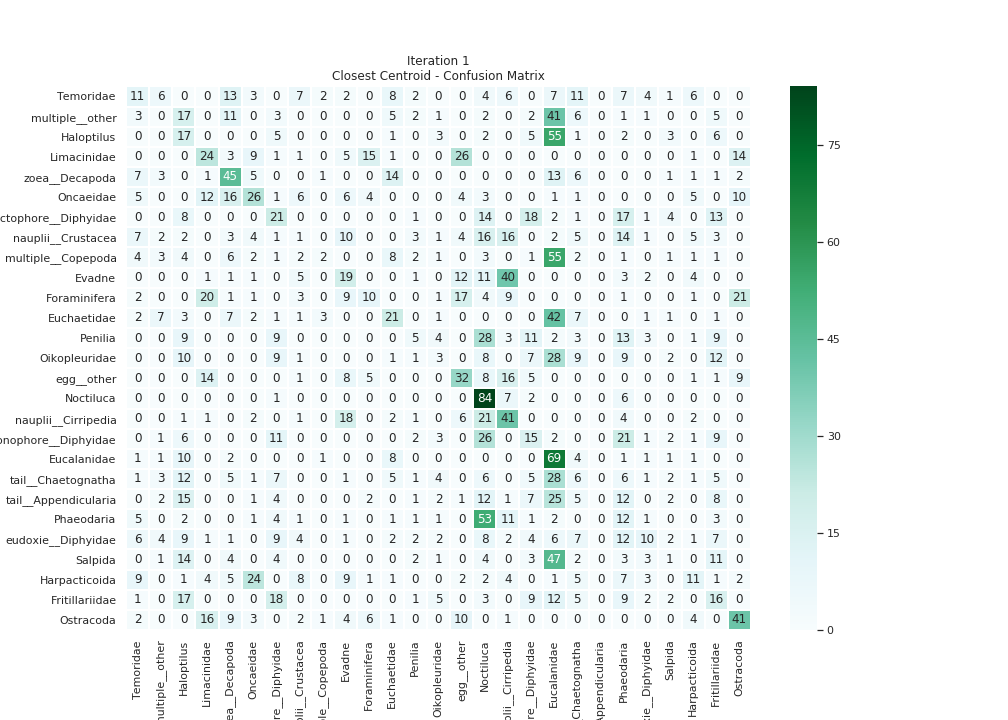
\includegraphics[scale=.5]{val_confusion_1.png}
\caption{Confusion @ 5 epochs. True class in rows, predicted in columns.}
\end{figure}

\begin{figure}
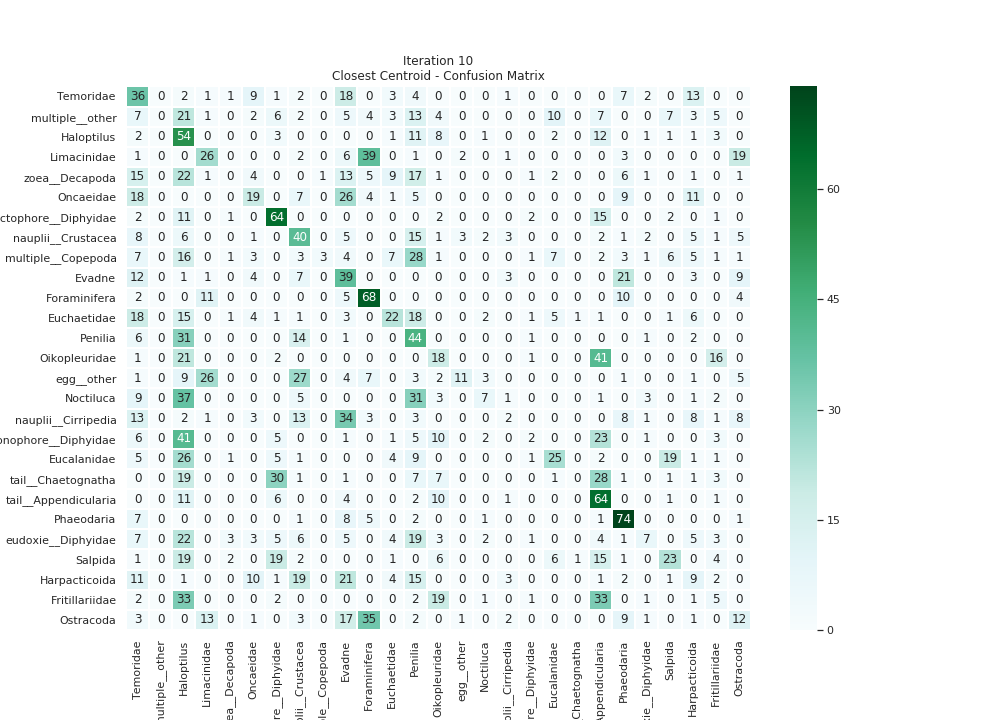
\includegraphics[scale=.5]{val_confusion_10.png}
\caption{Confusion @ 50 epochs. True class in rows, predicted in columns.}
\end{figure}

\begin{figure}
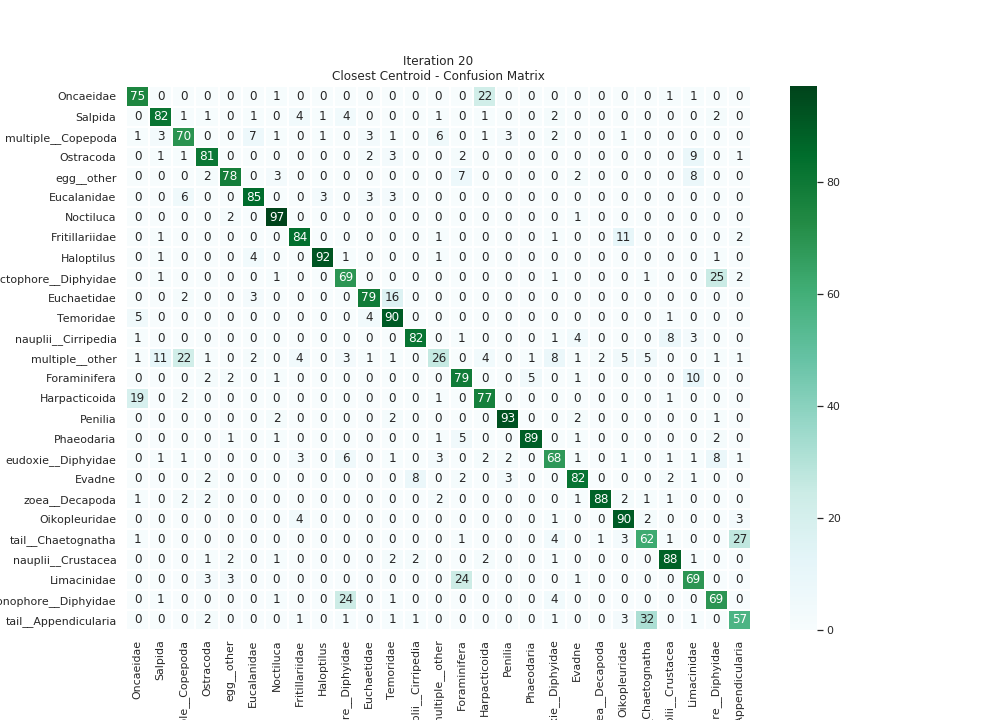
\includegraphics[scale=.5]{val_confusion_20.png}
\caption{Confusion @ 100 epochs. True class in rows, predicted in columns.}
\end{figure}

The training also provides periodic summaries showing the intra class centroid distances after each iteration as well as cluster sizes. As the centroid distance to itself is always zero, the diagonal of these plots is instead used to describe the cluster sizes.

\begin{figure}
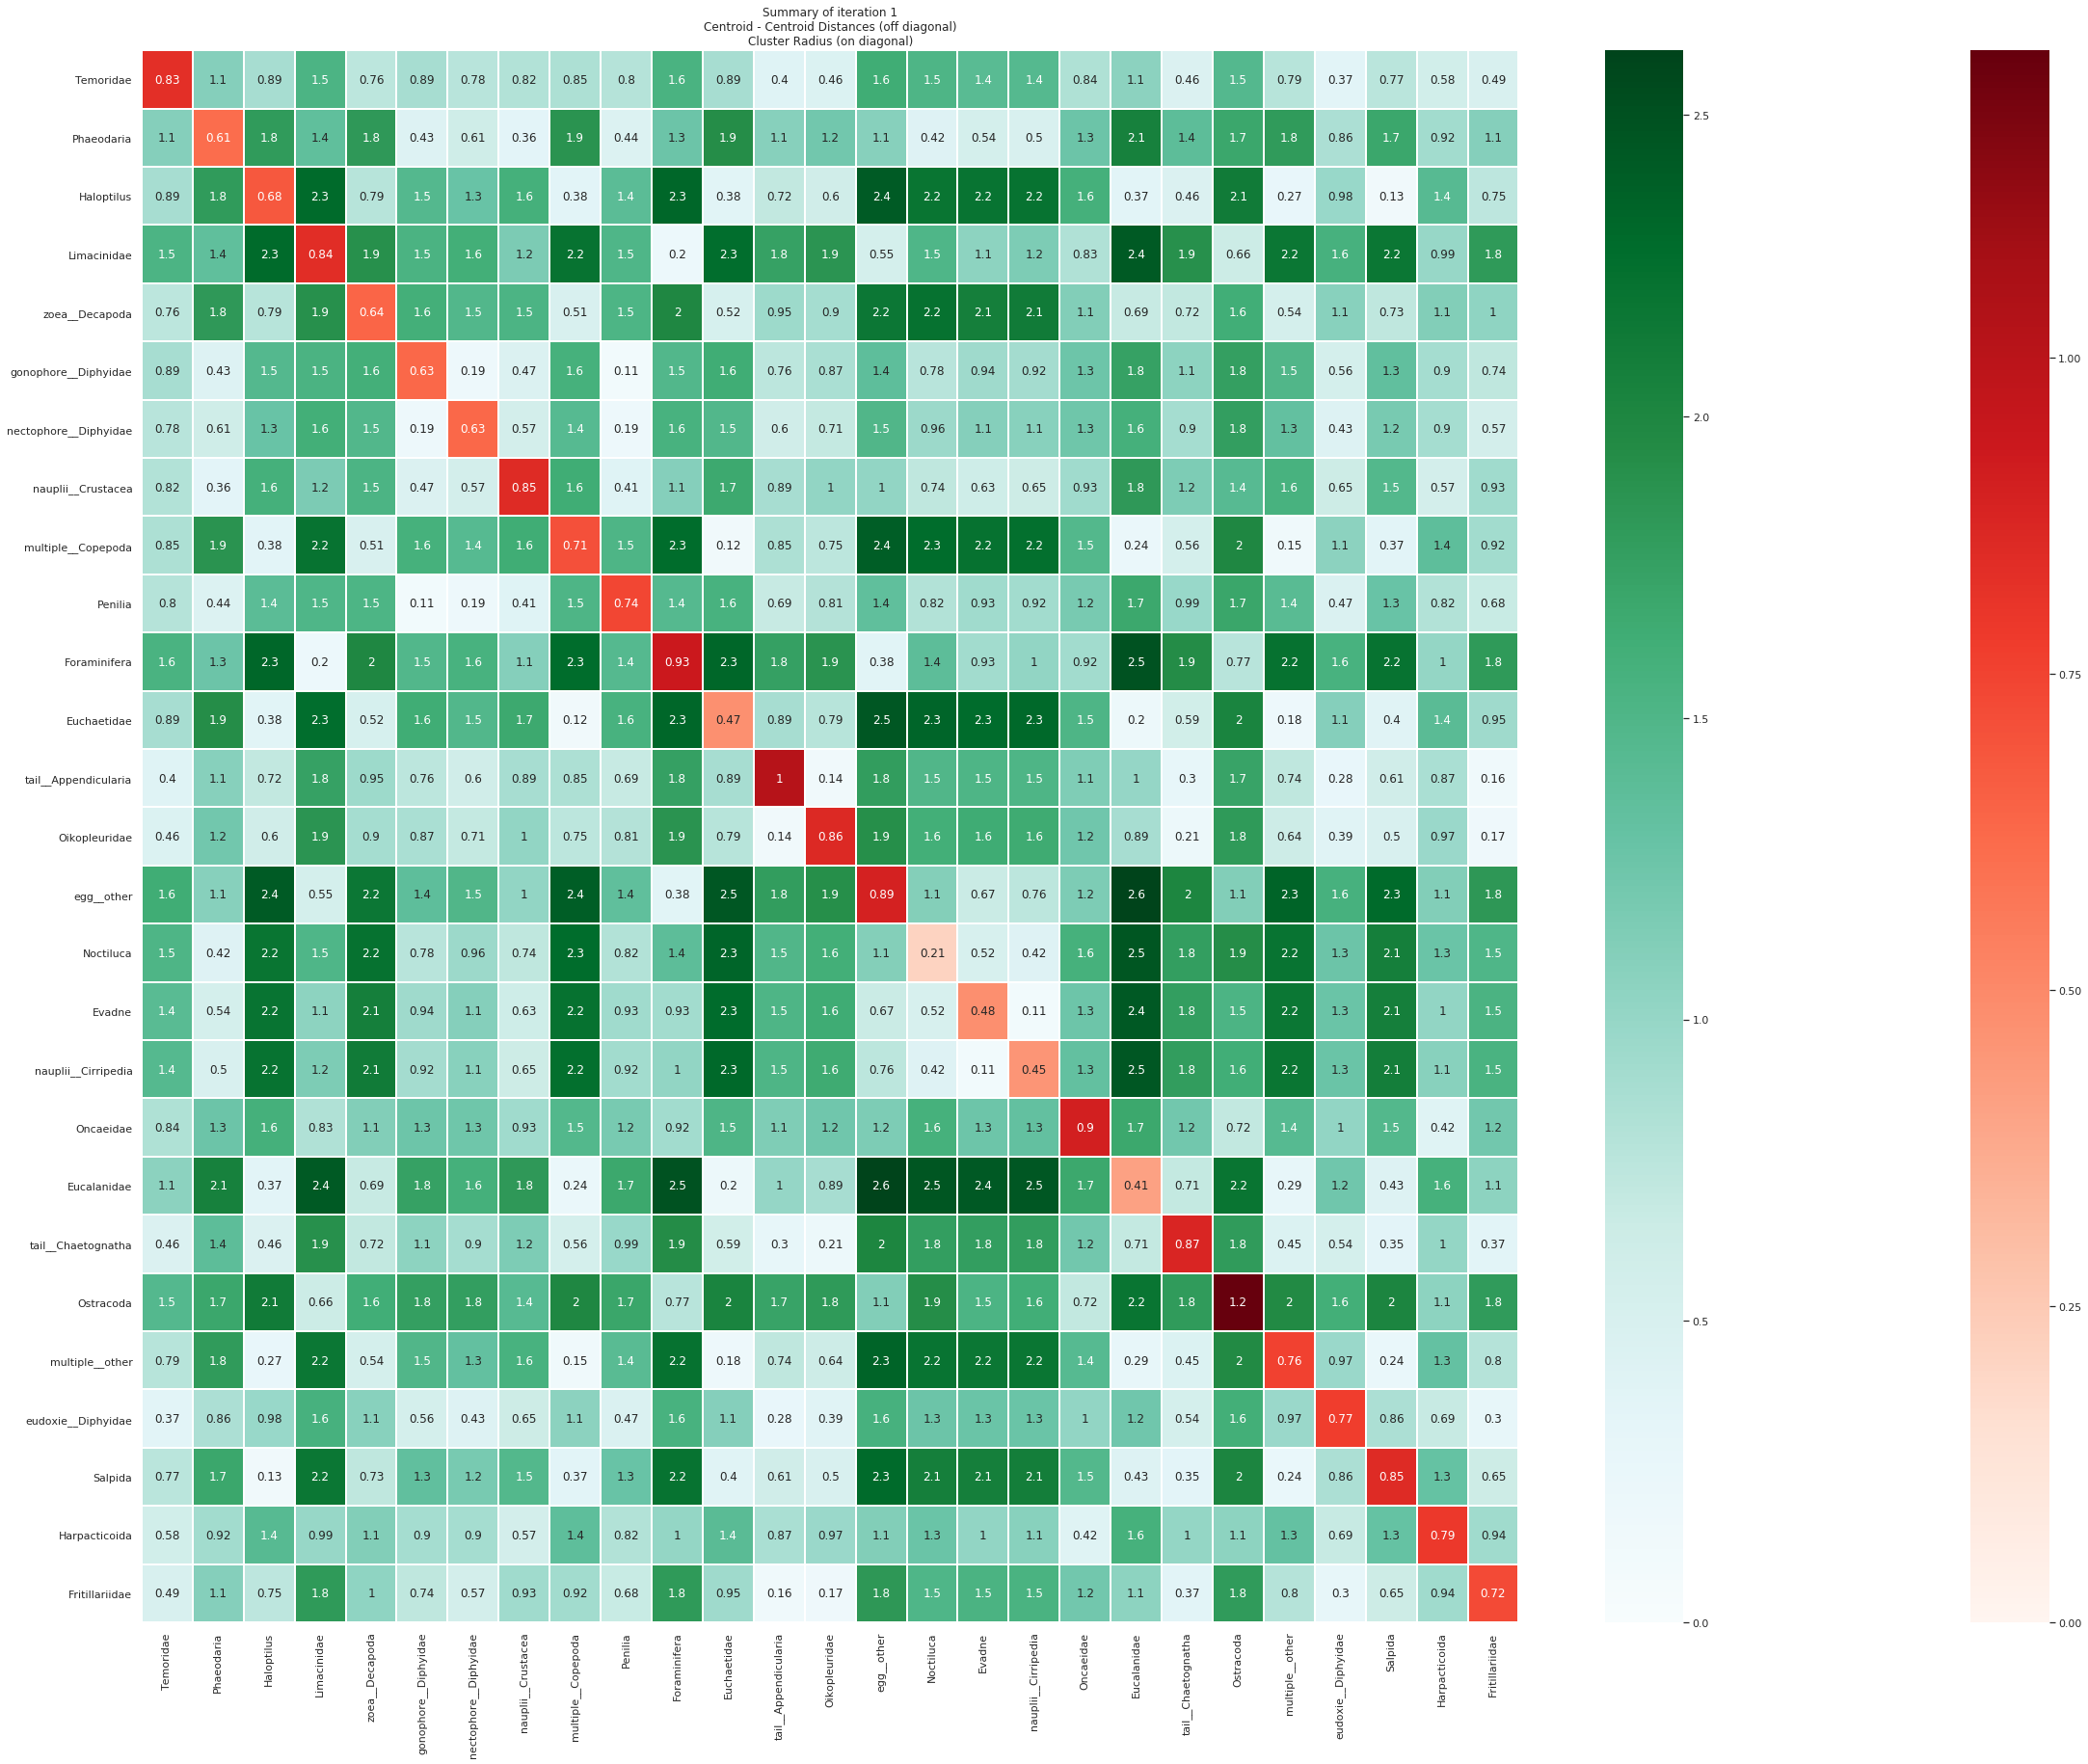
\includegraphics[angle=90, scale=.22]{summarize1.png}
\caption{Centroid distances @ 5 epochs. Cluster sizes on diagonal.}
\end{figure}

\begin{figure}
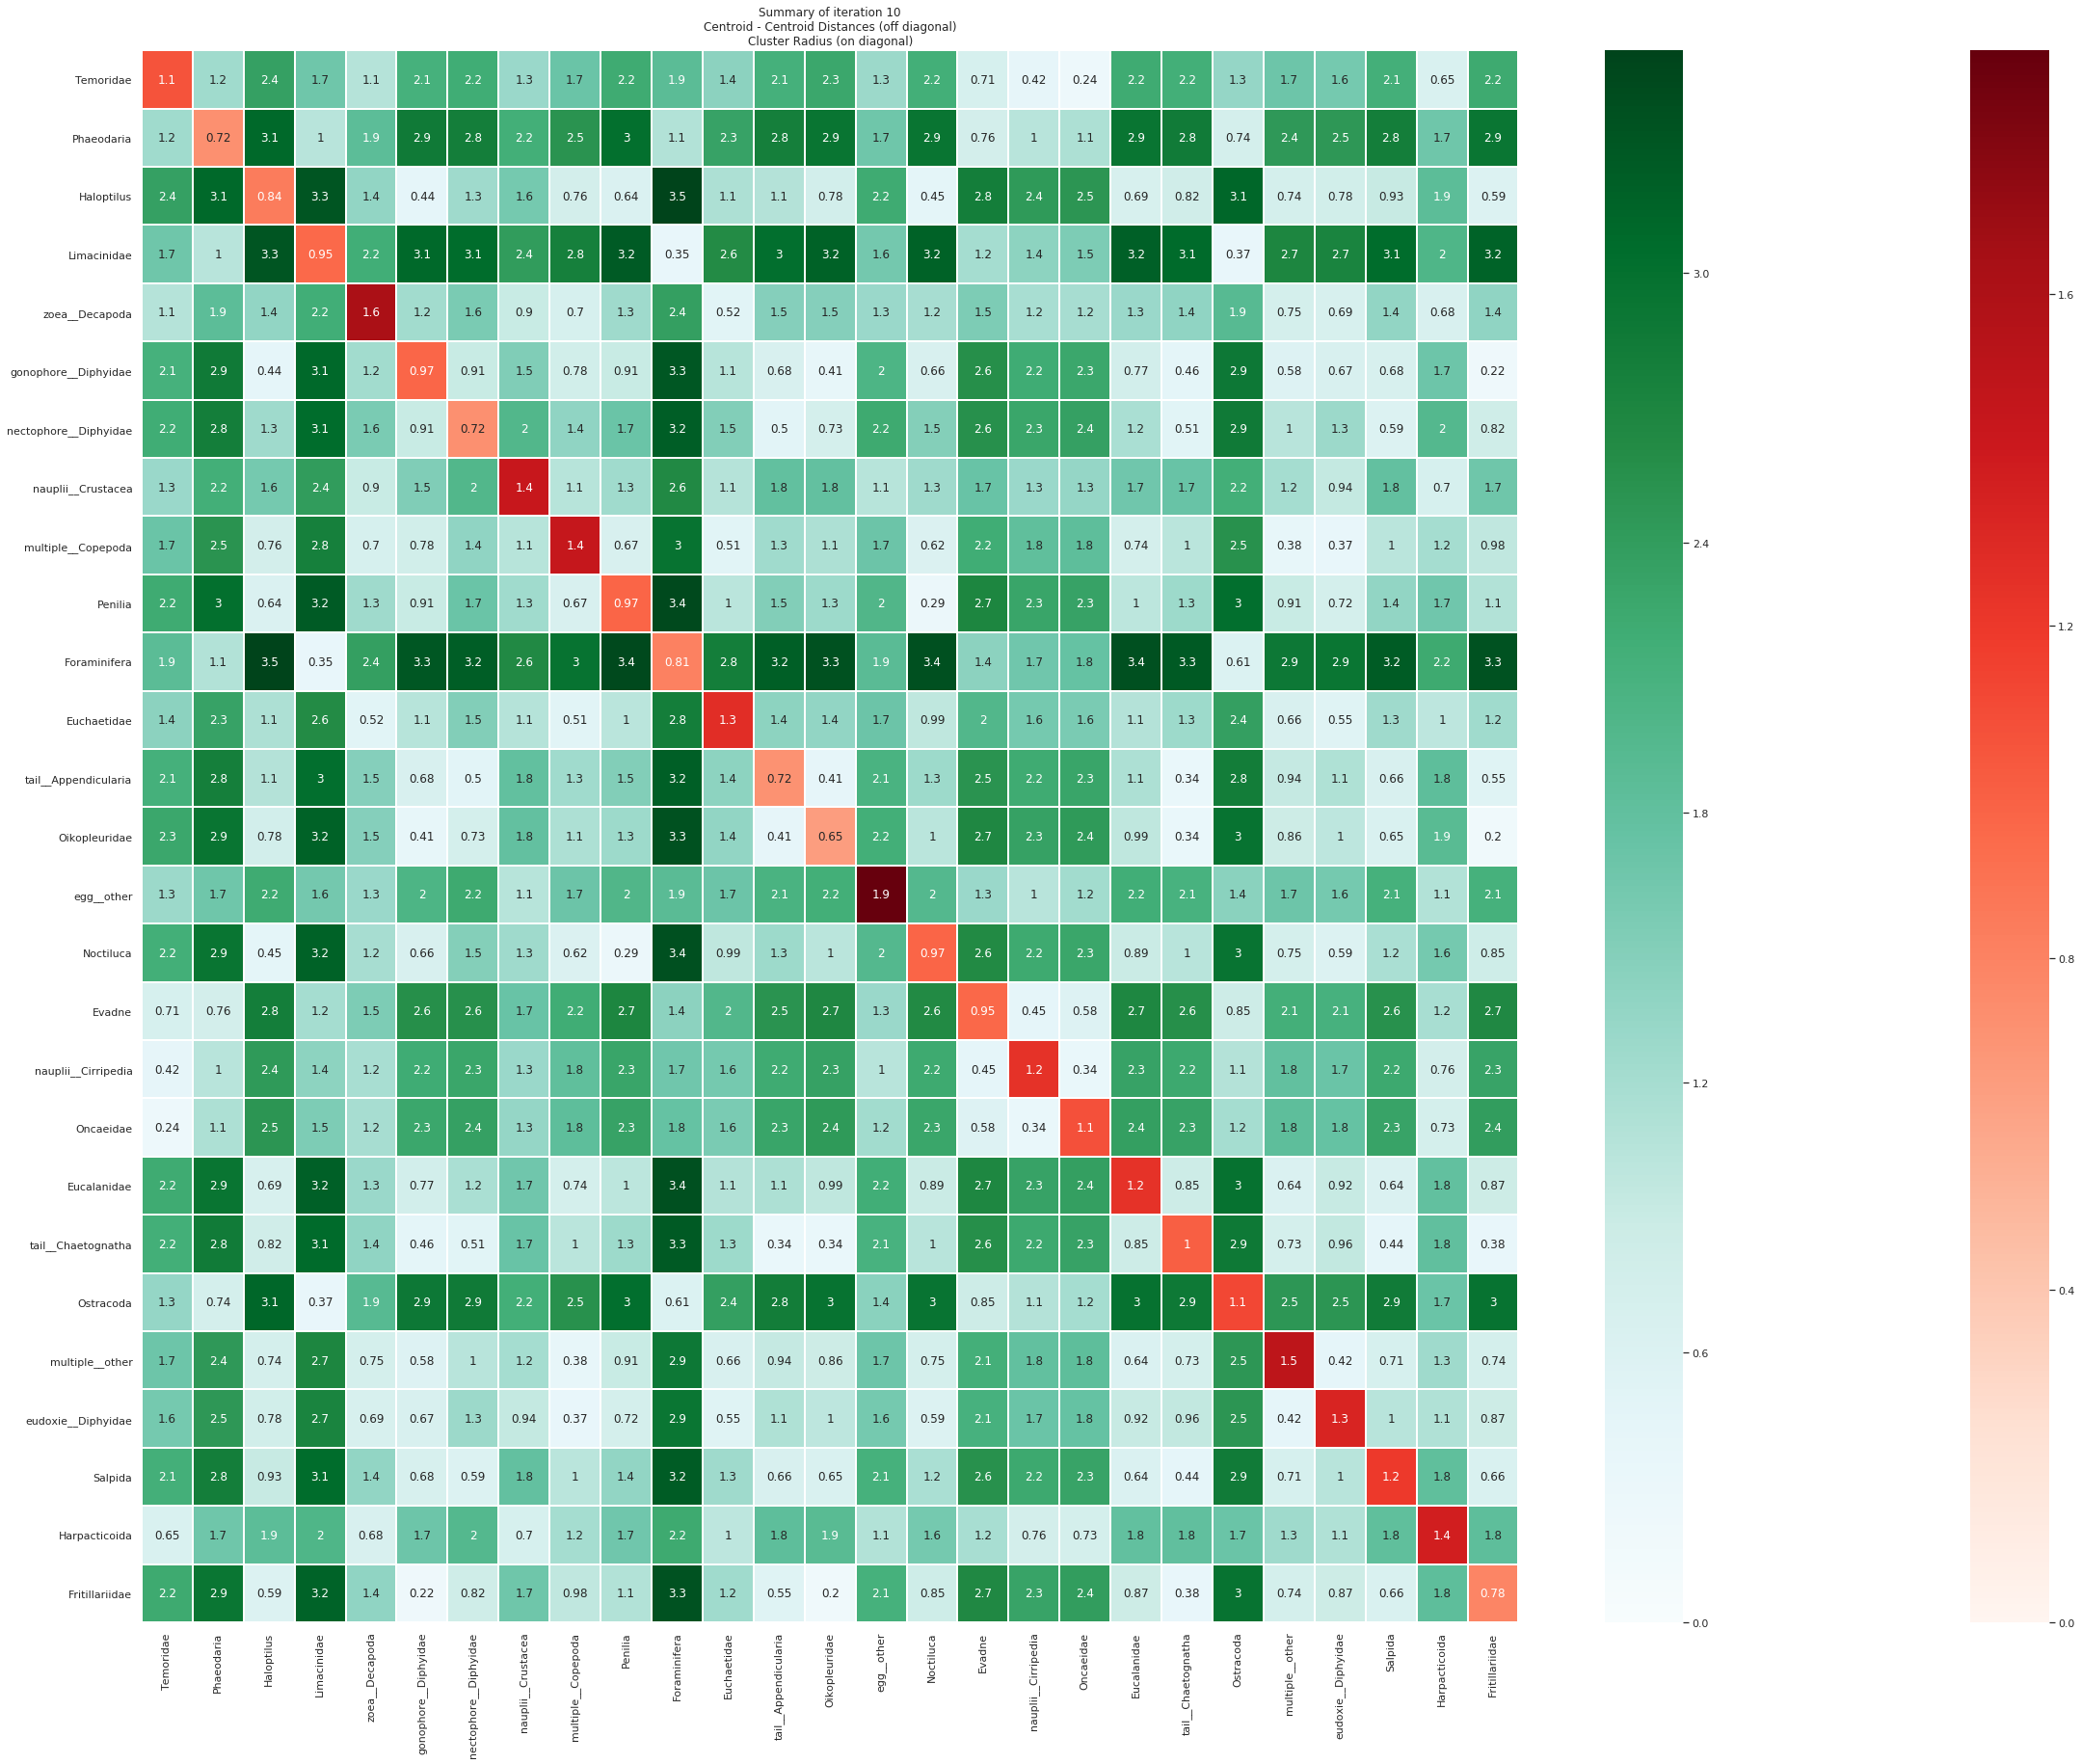
\includegraphics[angle=90, scale=.22]{summarize10.png}
\caption{Centroid distances @ 50 epochs. Cluster sizes on diagonal.}
\end{figure}

\begin{figure}
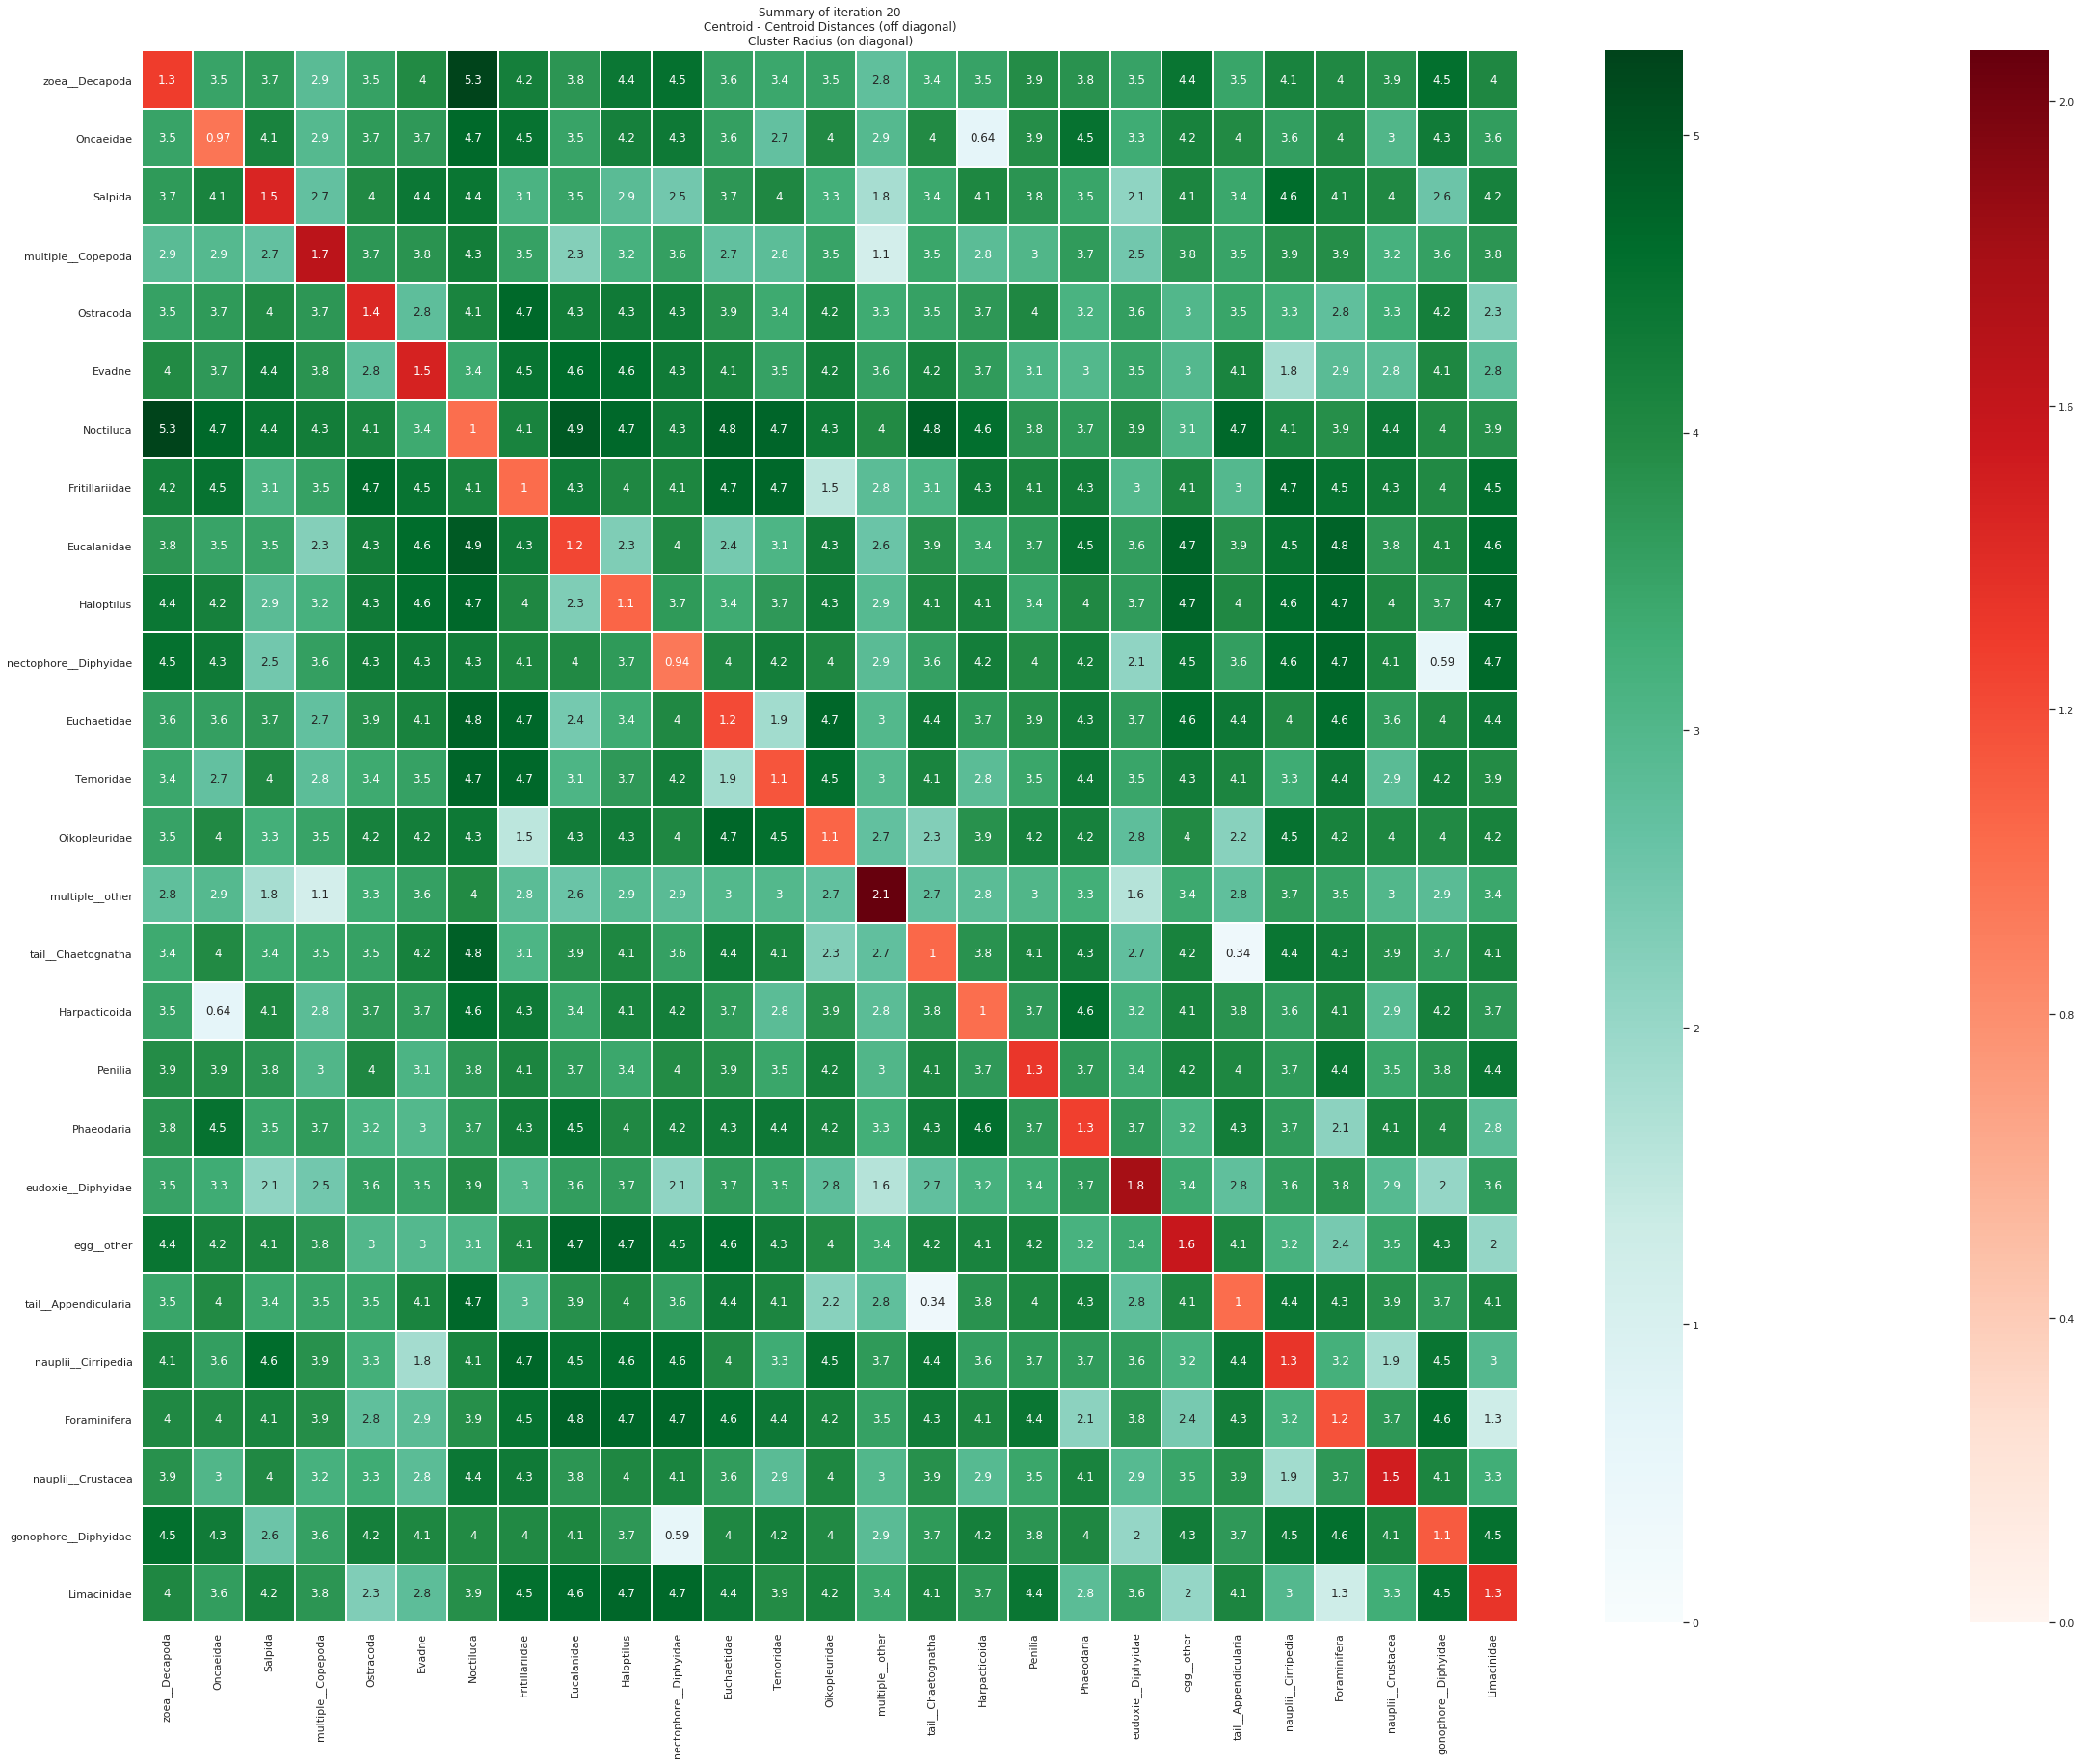
\includegraphics[angle=90, scale=.22]{summarize20.png}
\caption{Centroid distances @ 100 epochs. Cluster sizes on diagonal.}
\end{figure}

Regarding the summaries, we want big distances (dark colors off the diagonal) and small cluster sizes (light colors on the diagonal). It's hard to discern a strong development in either between the two first plots. A quick look at the time progression of the mean cluster size and centroid distance data confirms this. 

When we look at the summary heatmap of centroid distances and cluster sizes for the final epoch, the trend seems to be towards more distance, while sizes do not seem to change all that much. Looking at the progression of the two there seems to be little development after about 75 epochs where the mean size seems to stabilize, while the mean distance may show a weak positive trend from 50-100 epochs though variance is high.

All in all there seems to be little purpose in continuing training further than the 100 epochs here. There is a noticeable shift in the training and validation loss at 50 epochs where training was restarted with the original training rate - leading to the conclusion that perhaps the learning rate decay could be less agressive throughout.

\begin{figure}
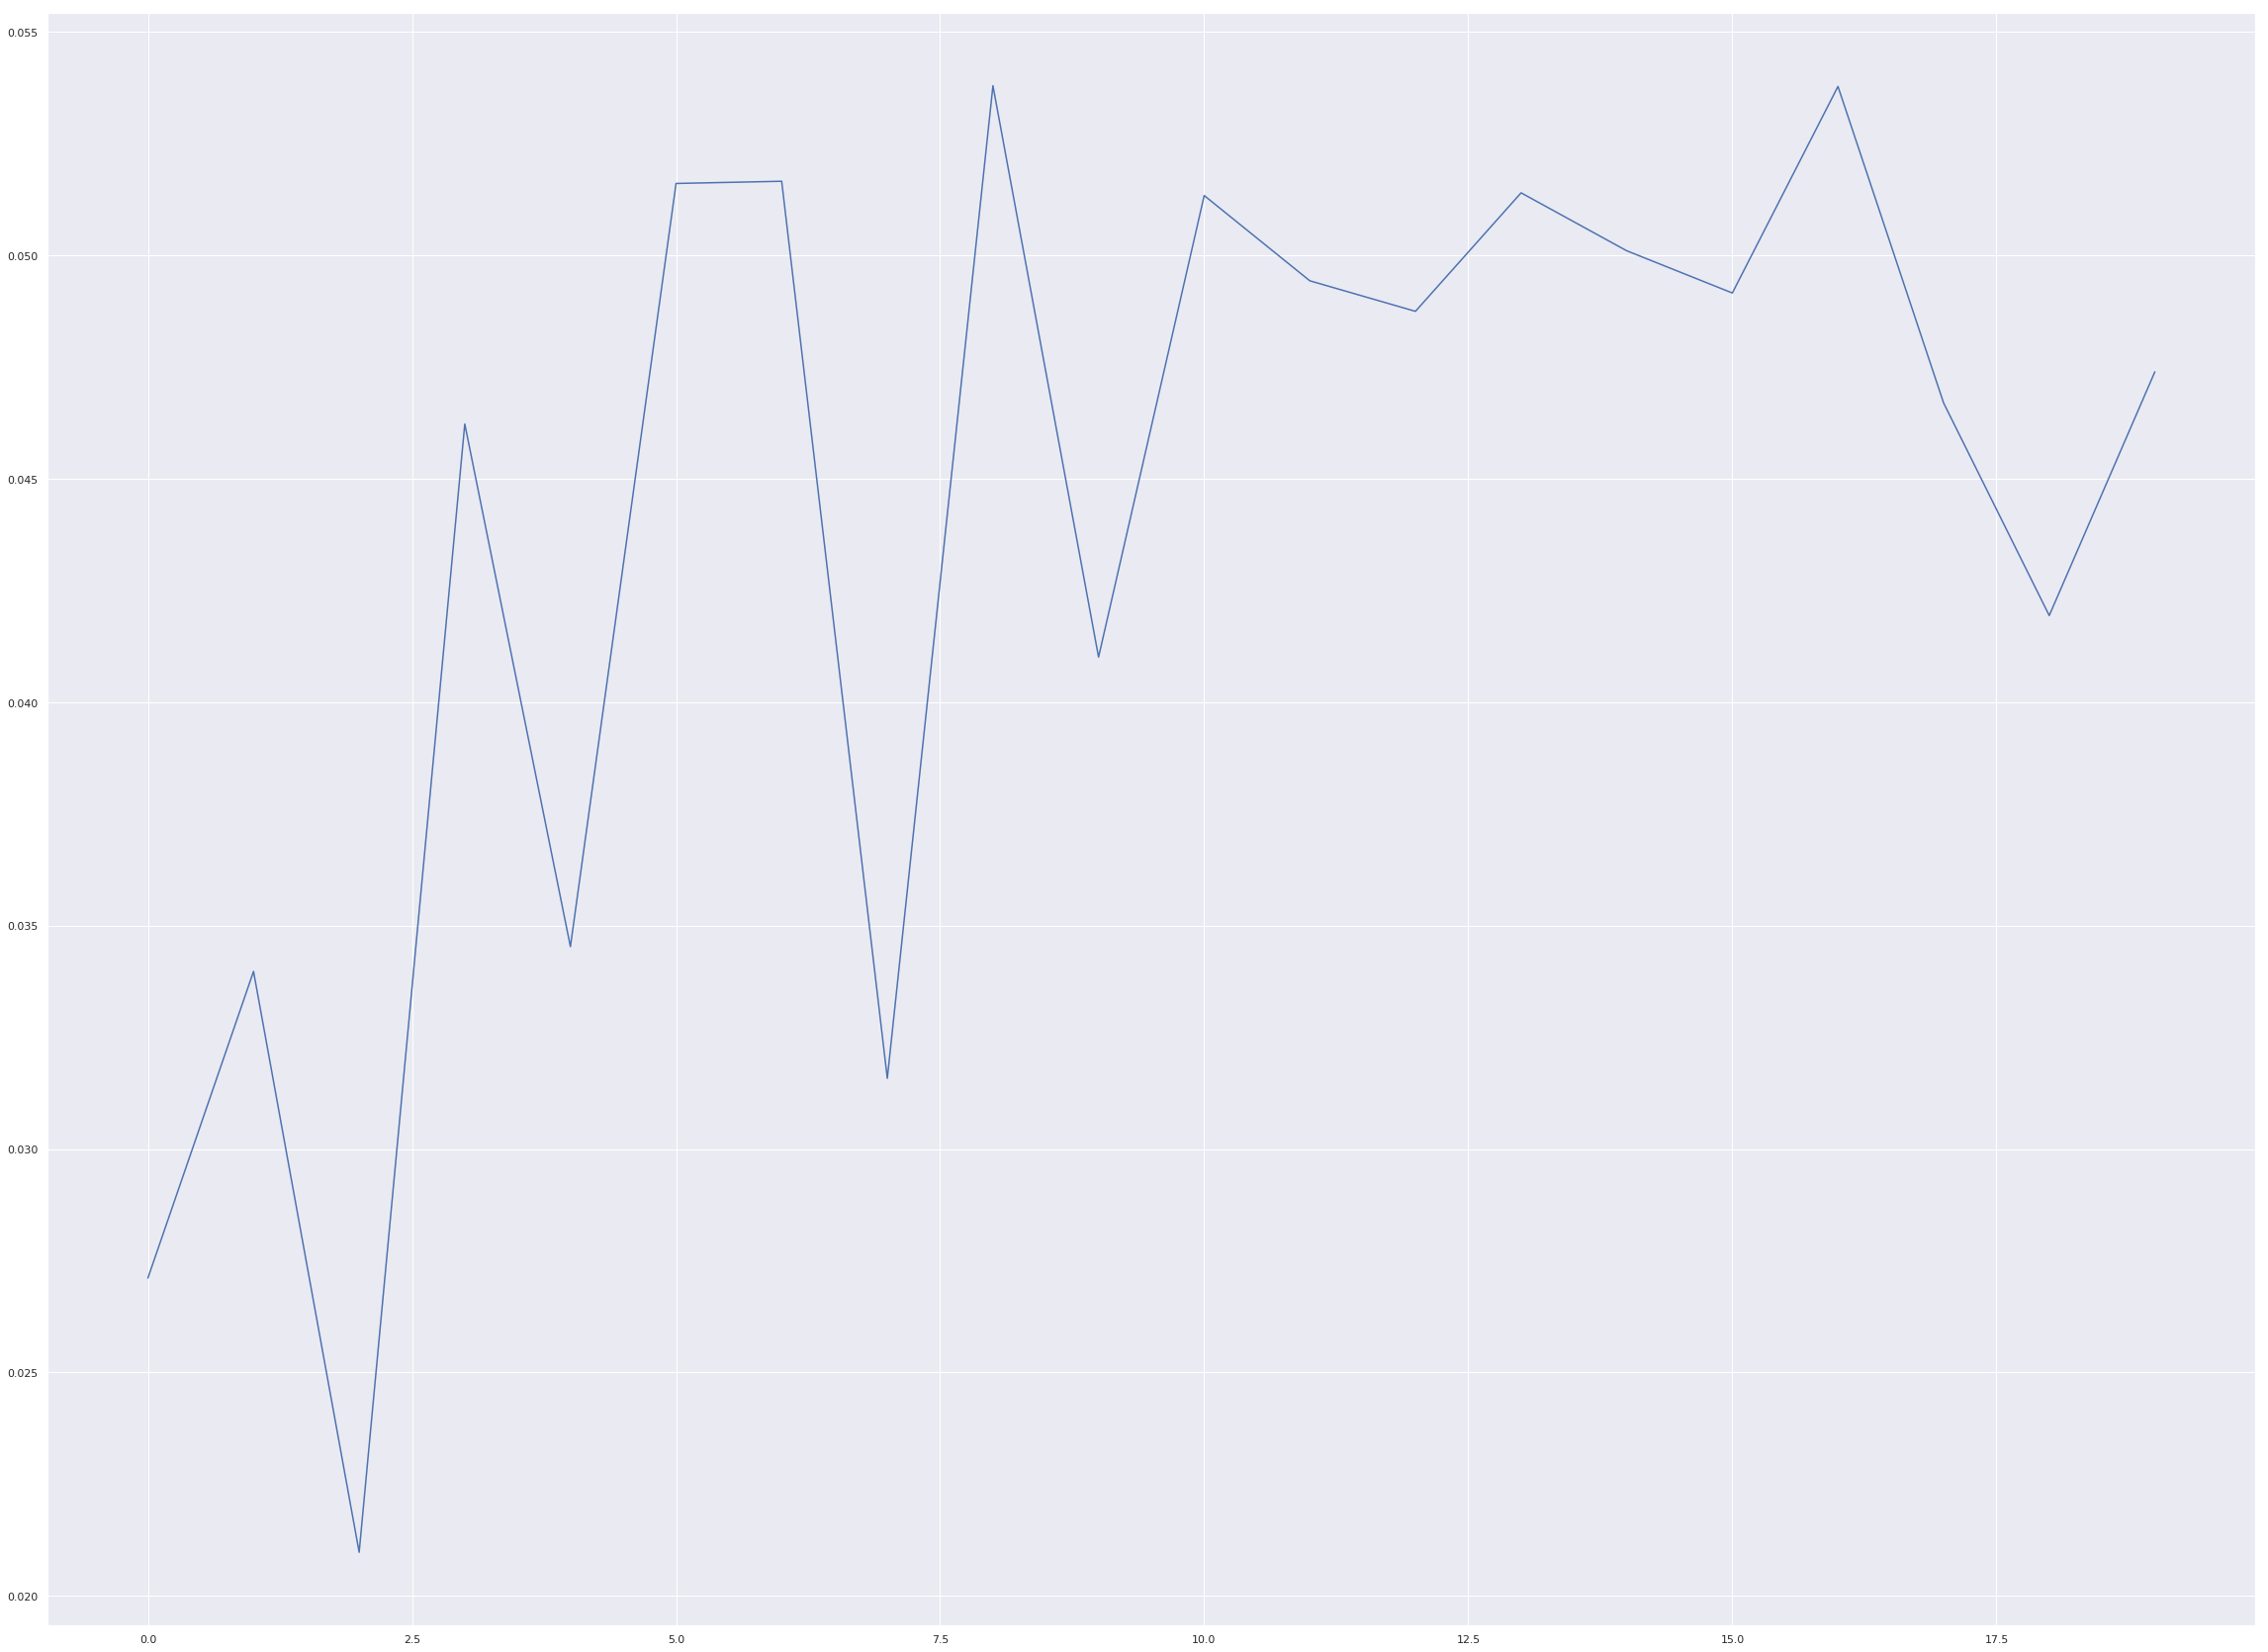
\includegraphics[scale=.15]{mean_size.png}
\caption{Mean cluster size progression over 100 epochs.}
\end{figure}

\begin{figure}
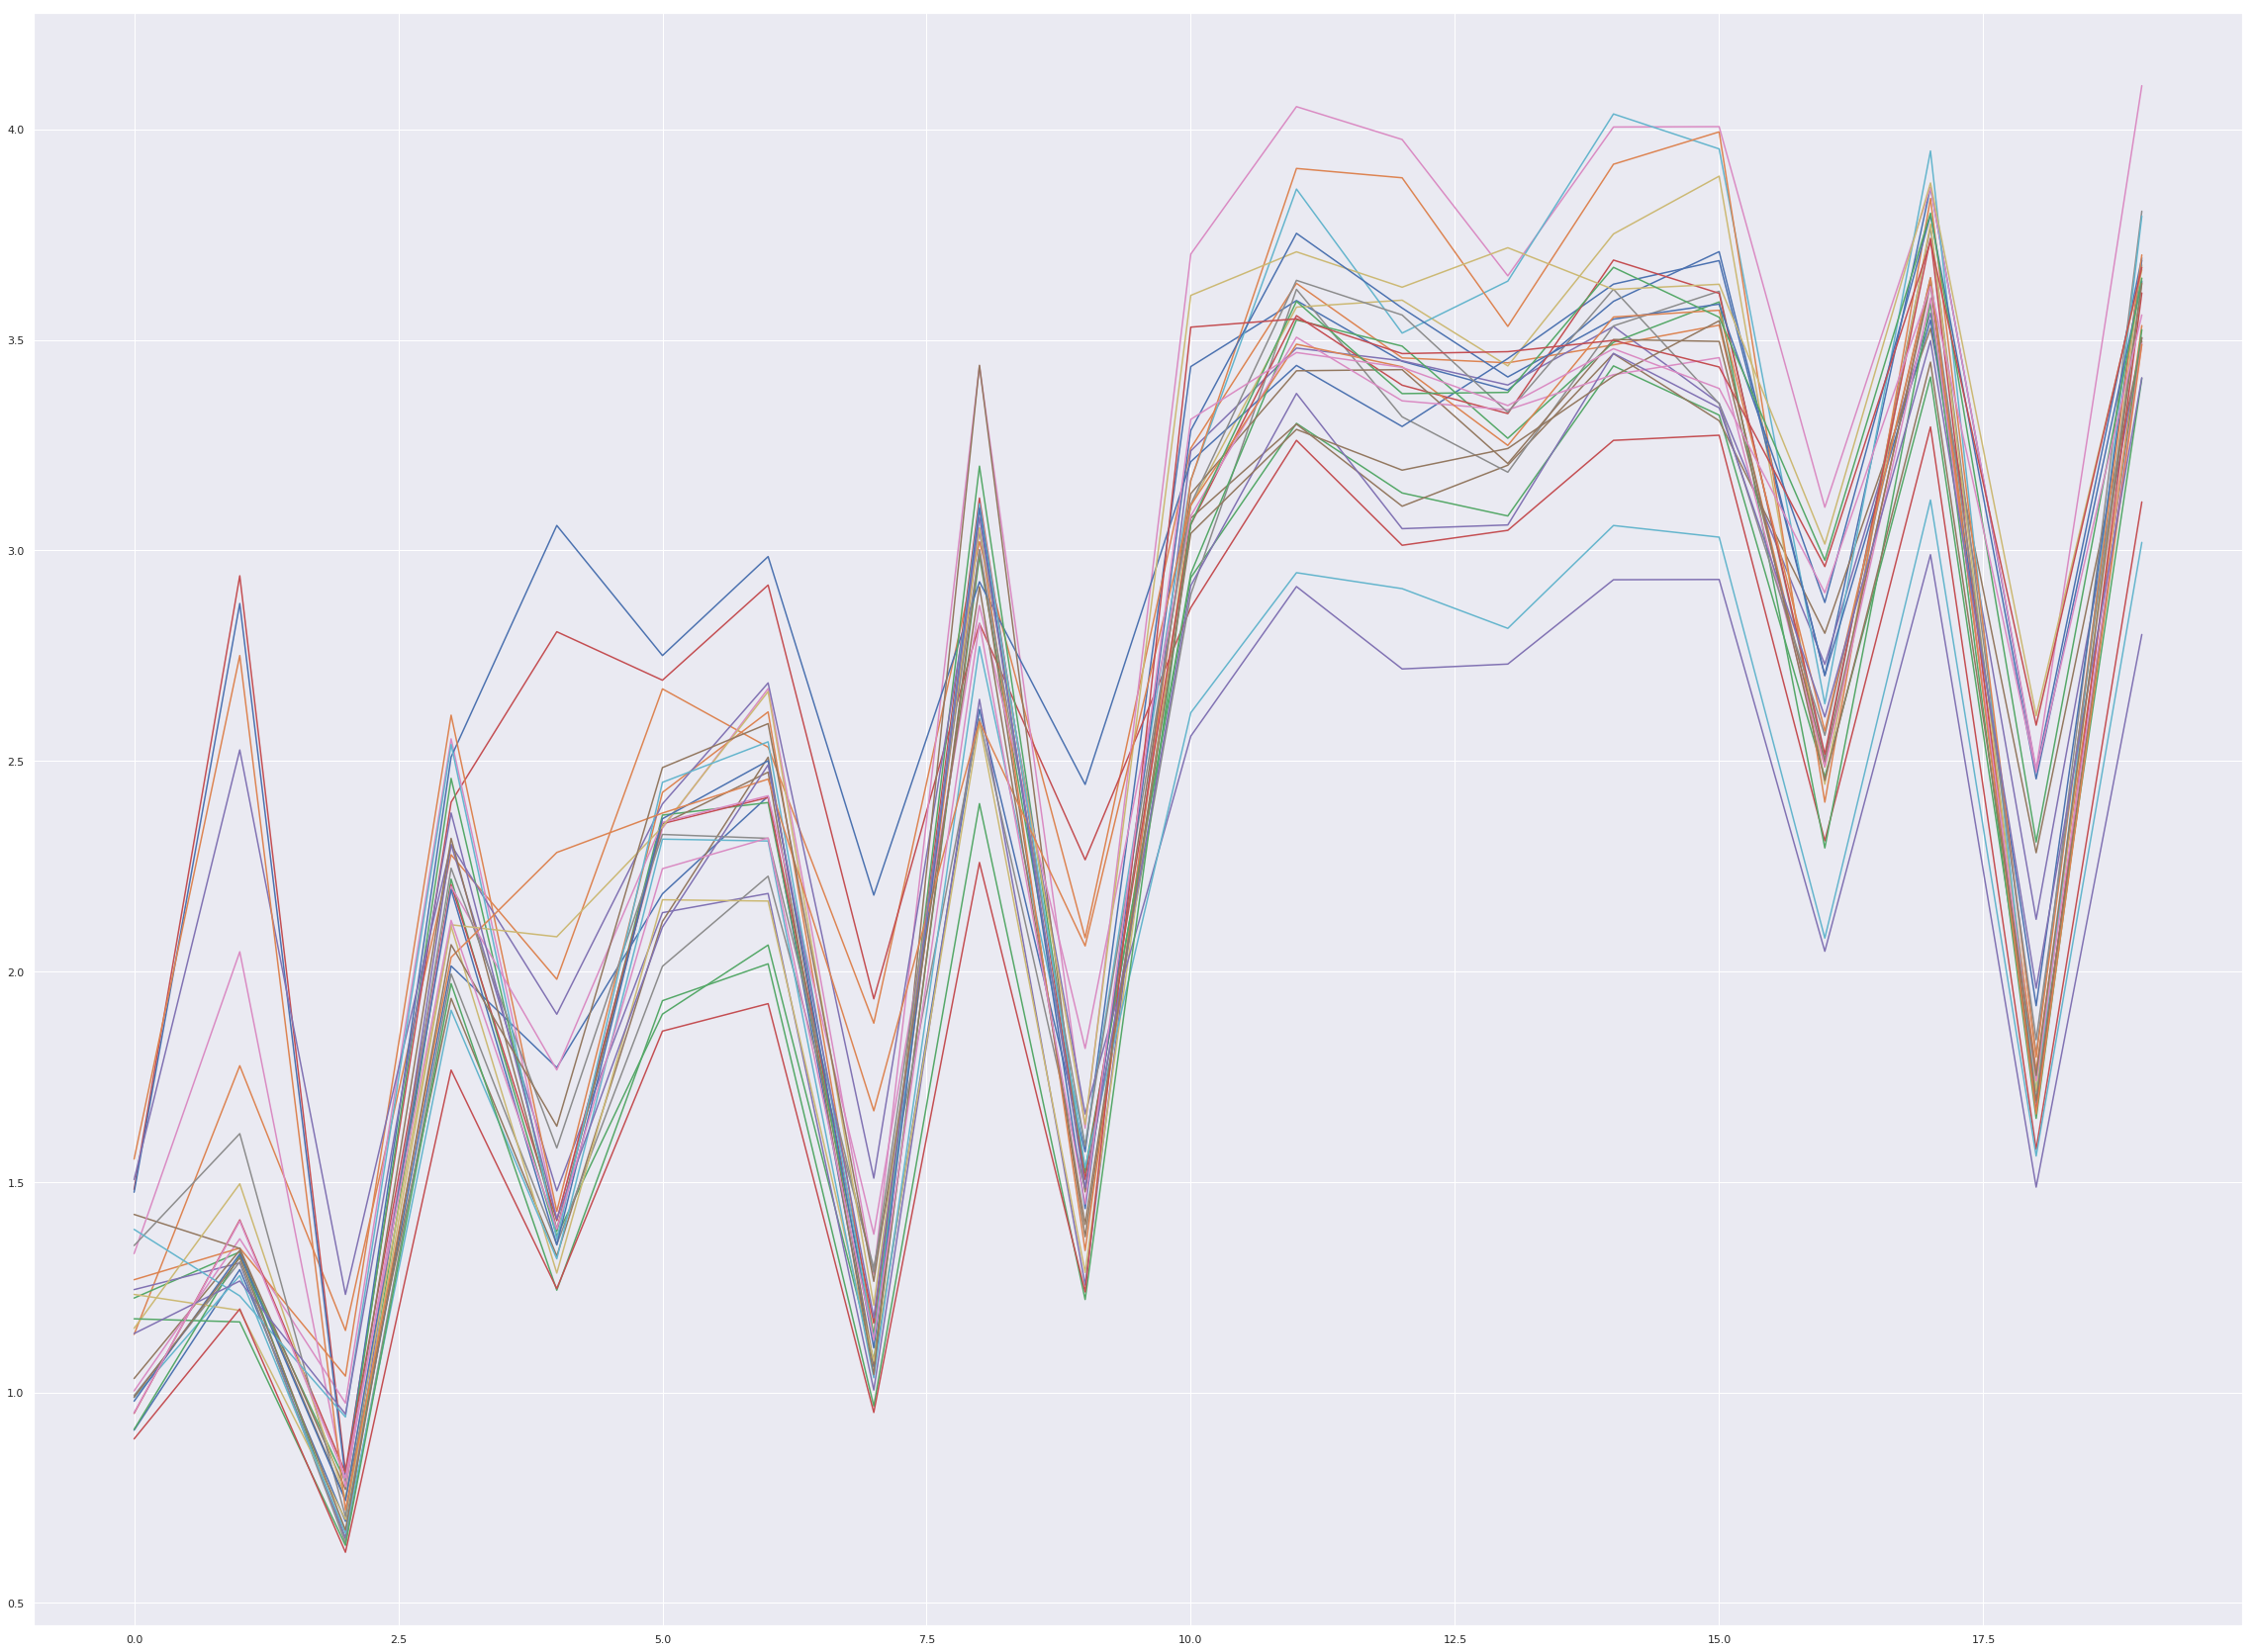
\includegraphics[scale=.15]{mean_dist.png}
\caption{Mean centroid distances progression over 100 epochs.}
\end{figure}

Finally we look at the training and validation losses as training progresses. Training loss decreases at a steady rate over the first 50 epochs used, while validation loss is more variable. For the last 50 epochs used, the validation loss also seems to plateau.

\begin{figure}
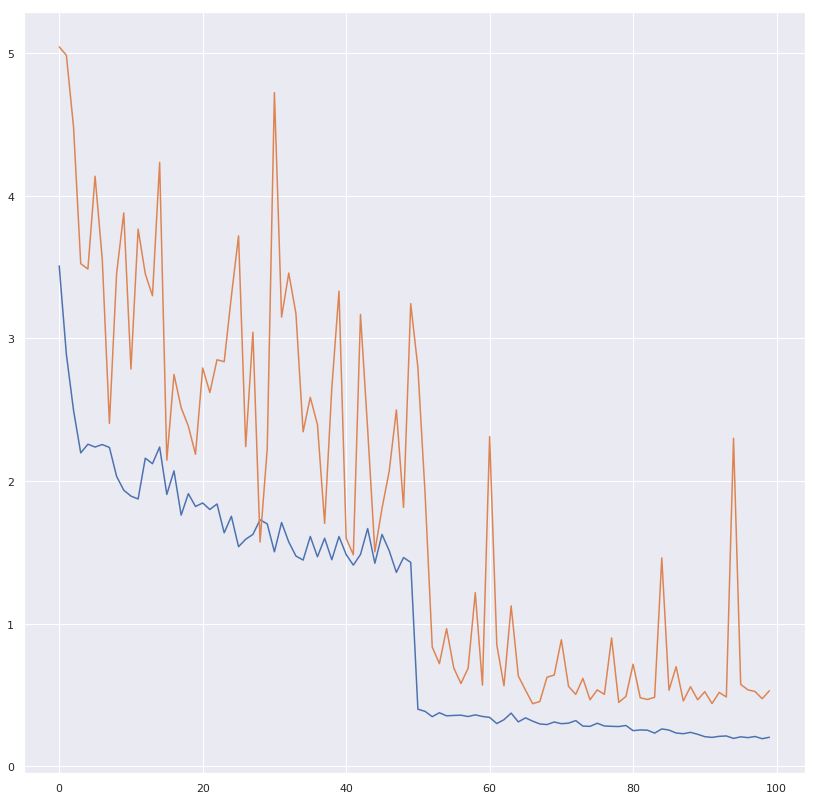
\includegraphics[scale=.45]{train_val_loss.png}
\caption{Training (blue) and validation (orange) losses over 100 epochs.}
\end{figure}

\section{Visualization}
Using the models generated during training, t-SNE visualizations were done for the validation data. At 50 epochs, The t-SNE visualization indicates some improvements in clustering of the data that is not clearly evident from the plots from the training section. At 100 epochs clustering is more evident, albeit with confusion between some classes being likely. Note in particular classes 24/25, classes 18/23 and 19/20. Though class numbers are used in the plots for clarity, these can easily be cross referenced in the confusion matrix plots below. The attached GIF animation illustrates how this develops over time.

The code for loading the models, running the vector embedding and finally creating and visualizing the t-SNE embedding can be found in the TSNE notebook in the GitHub repository referred above.

\begin{figure}
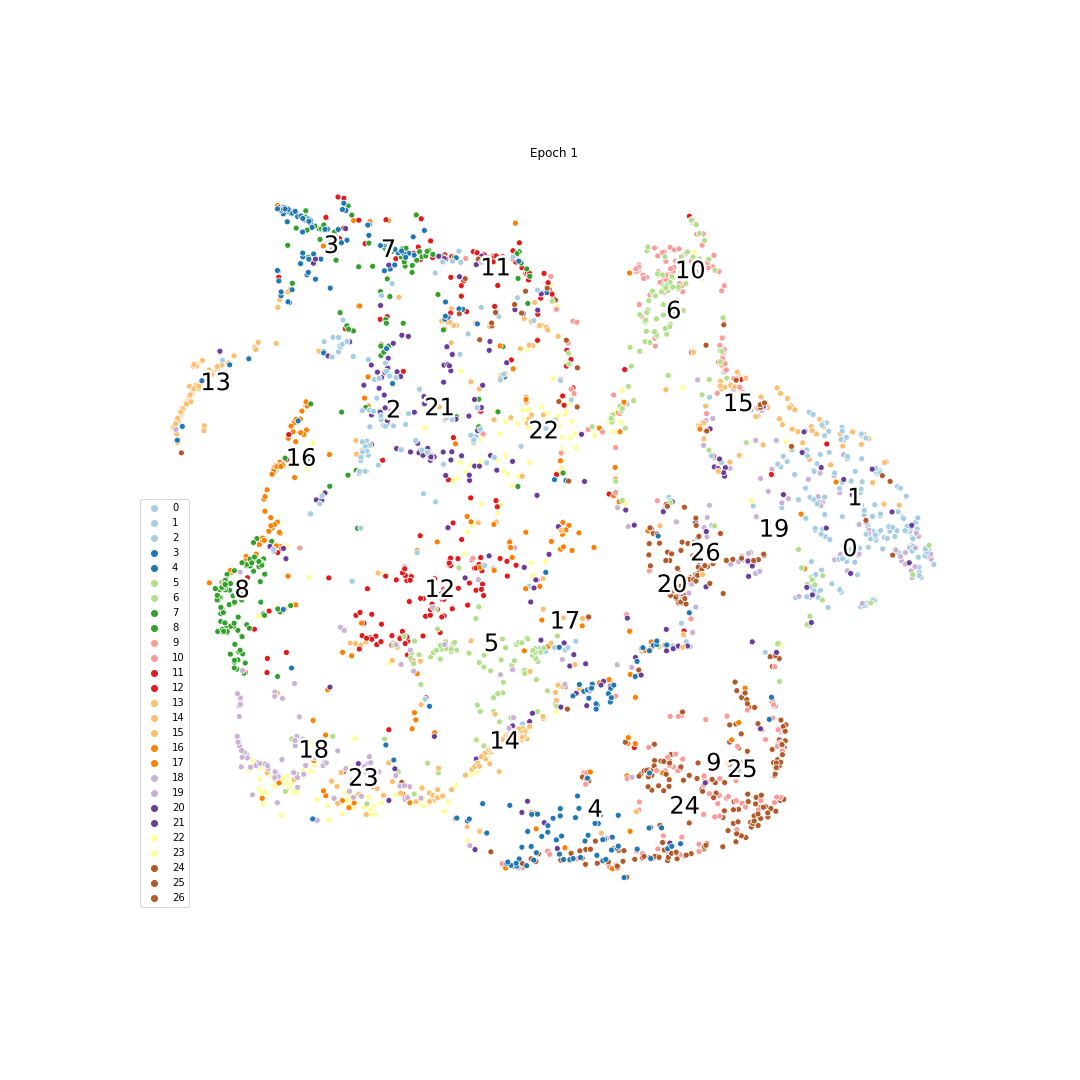
\includegraphics[scale=.45]{tsne/epoch_1.png}
\caption{t-SNE visualization after 5 epochs}
\end{figure}

\begin{figure}
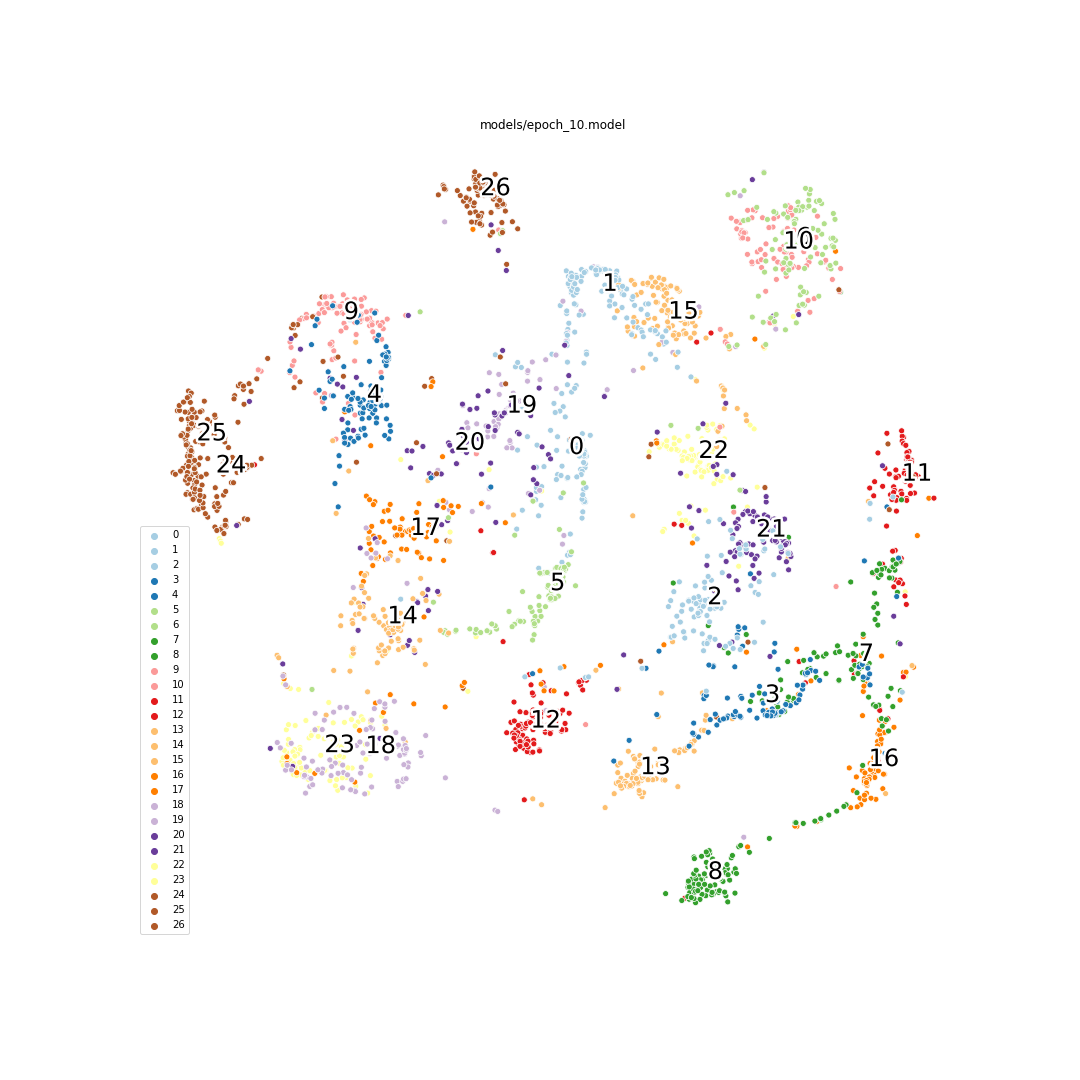
\includegraphics[scale=.45]{tsne/epoch_10.png}
\caption{t-SNE visualization after 50 epochs}
\end{figure}

\begin{figure}
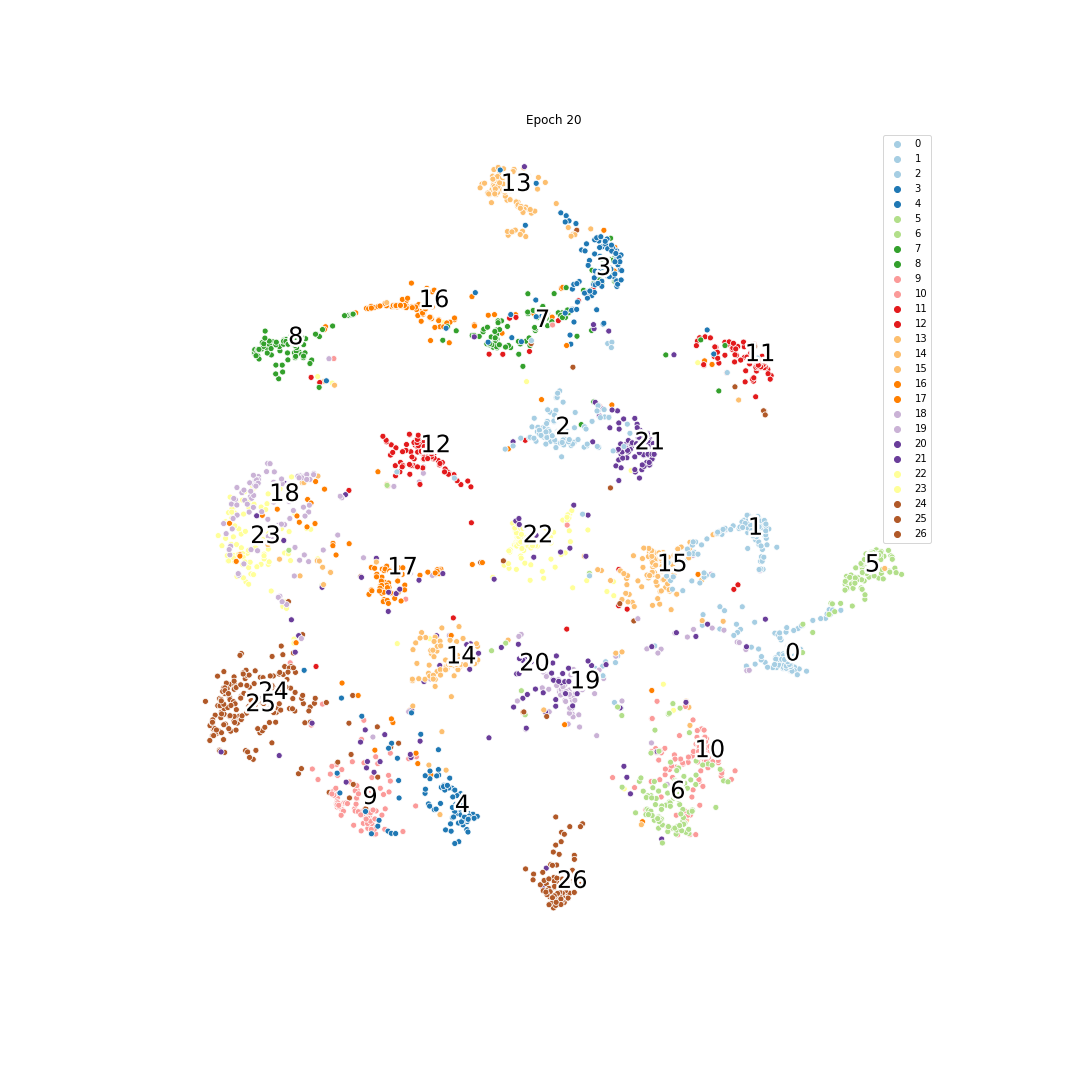
\includegraphics[scale=.45]{tsne/epoch_20.png}
\caption{t-SNE visualization after 100 epochs}
\end{figure}

\section{Classification}
For the classification, we base the following on embeddings of the images rather than the actual images. The embeddings correspond to the vectors returned by the final model from above.

Two separate classification schemes were set up. First among these was a support vector machine with a 3rd degree polynomial kernel. The classifier was fit to the validation data, and used to predict the class of the test data.

The classifiers are available in the \emph{Classifier} notebook in the code repository.

\begin{figure}
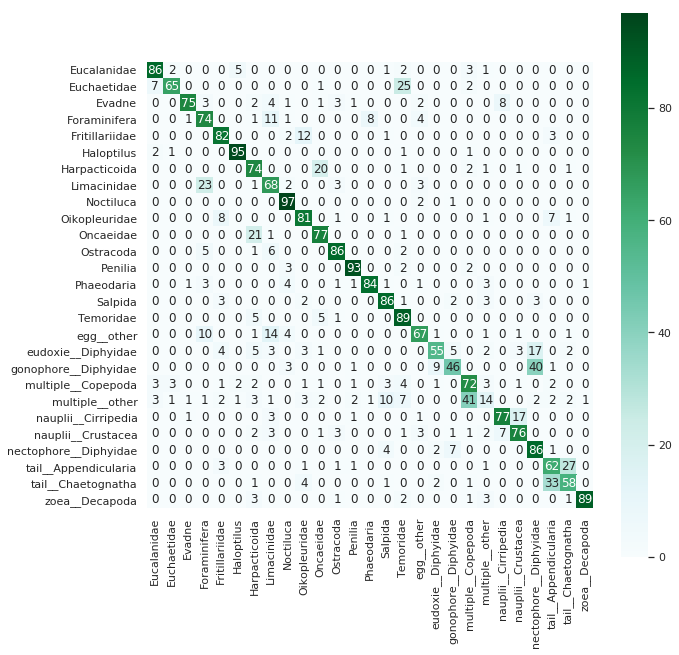
\includegraphics[scale=.55]{svm_acc.png}
\caption{SVM Confusion Matrix. True class in rows, predicted in cols.}
\end{figure}

\begin{figure}
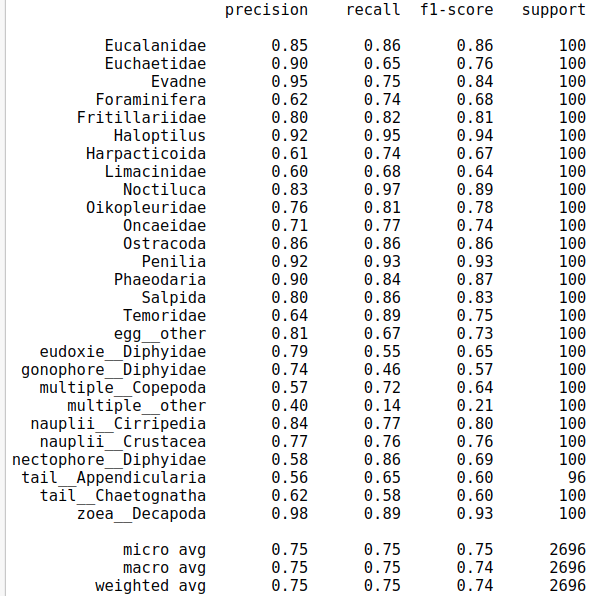
\includegraphics[scale=.55]{svm_crep.png}
\caption{SVM Classification Report}
\end{figure}

For an unsupervised approach, k-means was chosen, using the MiniBatchKMeans implementation from scikit-learn, with 27 clusters corresponding to the classes of our data. A challenge with evaluating the unsupervised learning is that the class of the data is not known, so it's not immediately apparent which cluster correspons to which class. To overcome this problem, the clustering algorithm was first fit to the validation data, then the test data was run through the prediction in a class-wise manner. The majority class of this prediction was then assumed to be predictive of the correct mapping between cluster number and actual class. We are thus able to produce a confusion matrix for the unsupervised case as well.

While the accuracy of the k-means clustering is slightly worse than that of the SVM classification, with 0.63 vs 0.75, it actually does a decent job for most of the classes. Some noteable exceptions occur, and it is of particular interest to note the confusion between the two tail classes - as this pops up in all our visualizations.

\begin{figure}
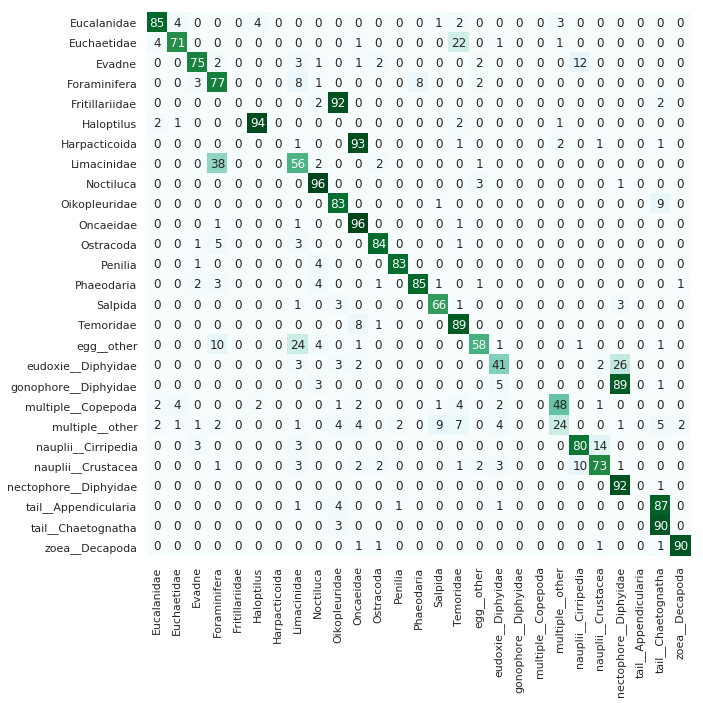
\includegraphics[scale=.55]{kmeans.png}
\caption{27-means clustering Confusion Matrix. True class in rows, predicted in cols.}
\end{figure}

\begin{figure}
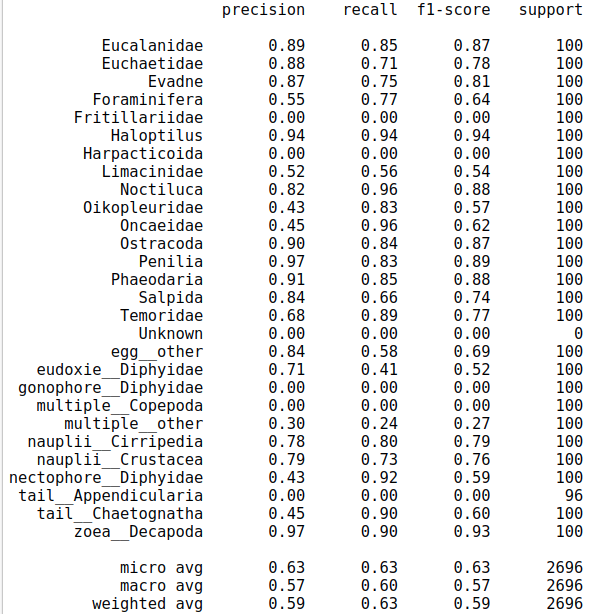
\includegraphics[scale=.55]{kmeans_crep.png}
\caption{k-means Classification Report}
\end{figure}

For an example of classes which are confounded in the classifiers, we can have a look at some samples from the classes \emph{tail\_\_Appendicularia} and \emph{tail\_\_Chaetognatha}. Clearly these are both tails, and visual inspection shows them to be similar in appearance as well. It is interesting to note that this is clearly reflected in both the t-SNE plot above, where classes 24 and 25 are quite close, and the confusion matrices of unsupervised or supervised classification run on the vector embeddings of the images.

\begin{figure}
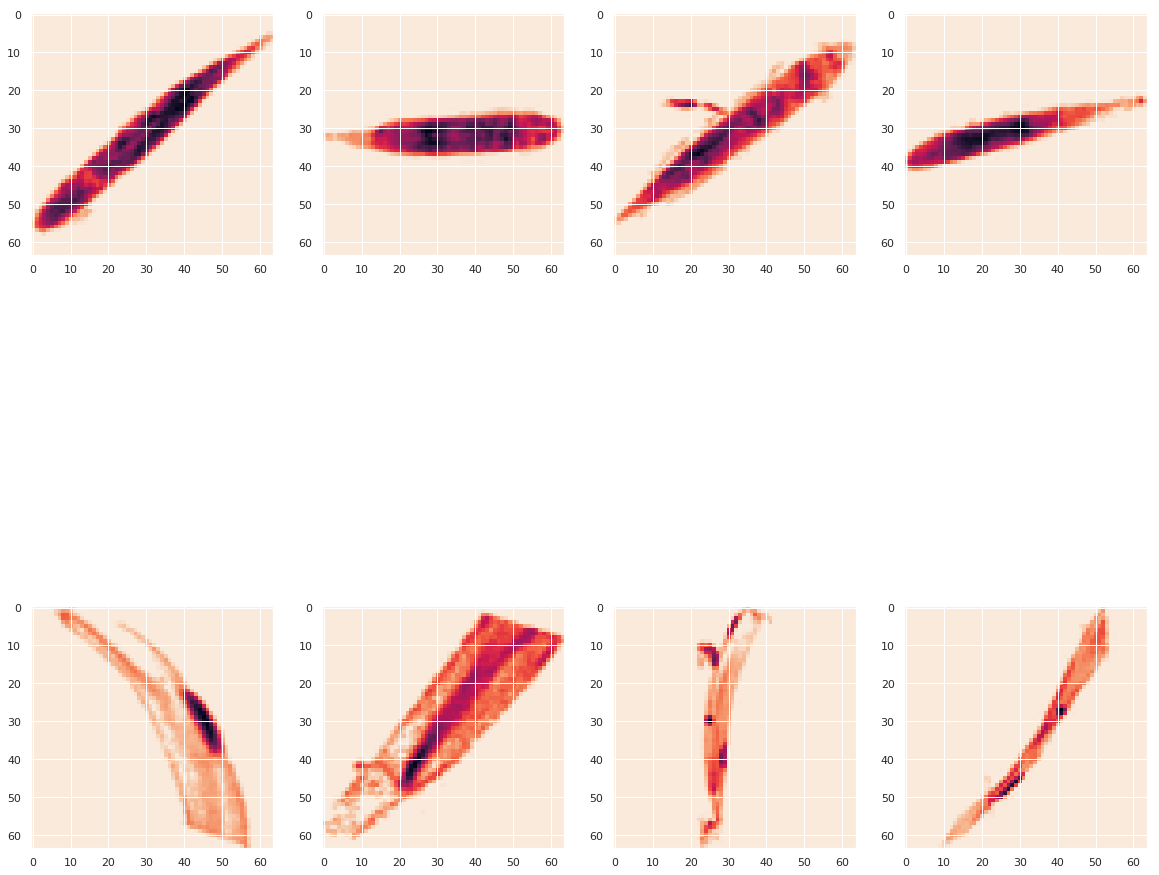
\includegraphics[scale=.35]{confusion_24_25}
\caption{Similarity between the classes tail-Appendicularia (above) and tail-Chaetognatha (below)}
\end{figure}

\end{document}
